% Appendix C

\chapter{Notaci\'on Actuarial} % Main appendix title

\label{AppendixC} % For referencing this appendix elsewhere, use \ref{AppendixA}
%\vspace{-1cm}
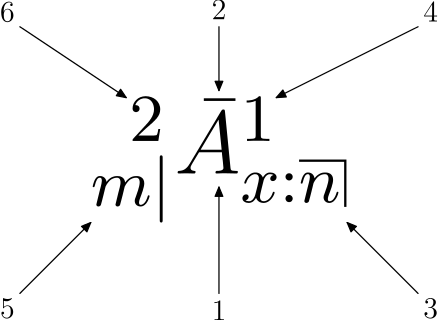
\includegraphics[scale=0.2]{Apendices/notation.png}\\

\noindent La renta vitalicia anual actuarialmente equivalente en los planes de aportaci\'on definida es:
$$F_{x_{j}}=\mathlarger{R}_{x_{j}}\ddot{a}_{x_{j}}}+\mathlarger{k}\mathlarger{R}_{x_{j}}\ddot{a}_{x_{j}|y}$$
donde:\\
\noindent 
\textbullet\ $x_{j}=$ Edad de jubilaci\'on del part\'icipe\\ 
\textbullet\ $\mathlarger{k}=$ Fracci\'on de la renta reversible al c\'onyuge del beneficiario cuya edad es $Y_{j}$\\ 
\textbullet\ $\ddot{a}_{x_{j}|y}=$ Valor actual actuarial de una renta anual unitaria de supervivencia\\\\ 
y como se vio, el modelo estoc\'astico viene especificado como la variable aleatoria 
$$Z=\text{VA (pensiones del titular y del c\'onyuge)}=Z_{1}+Z_{2}$$ 
Si se consideran las variables aleatorias (rentas unitarias):\\\\ 
\textbullet\ $Z_{1}$, \textbf{correspondiente al titular}, cuyo espacio num\'erico es $\{\ddot{a}\angle{t}_{i}$\}, siendo el tiempo de supervivencia $t=1,2,...,\omega - y$ y con funci\'on de probabilidad $P[Z_{1}=\ddot{a}\angle{t}_{i}]=\ _{t|}q_{x_{j}}$\\
\textbullet\ $Z_{2}$, \textbf{correspondiente a la pensi\'on de supervivencia} del c\'onyuge y con espacio muestral $k v^{t}\ddot{a}_{y_{j}+t}$, $t=1, 2,...,\omega - y$ y con funci\'on de probabilidad $P[Z_{2}=k v^{t}\ddot{a}_{y_{j}+t}]=\ _{t-1|}q_{x_{j}}\ _{t}p_{y_{j}}$\\\\
A partir de estas distribuciones de $Z_{1}$ y $Z_{2}$, se obtiene:\\\\
$E[Z]=E(Z_{1})+E(Z_{2})=\ddot{a}_{x_{j}}+k\ \ddot{a}\angle{x_{j}}_{y_{j}}$\\
$\sigma^{2}(Z)=\sigma^{2}(Z_{1})+\sigma^{2}(Z_{2})+2 Cov(Z_{1} Z_{2})$\\\\ 
y donde\\\\
$\sigma^{2}(Z_{1})=\mathlarger{\sum}\limits_{t=0}^{\omega-x_{j}}\big[\ddot{a}\angle{t+1}_{i}\big]^{2}\ _{t|} q_{x_{j}}-\big[\ddot{a}_{x_{j}}\big]^{2}$\\
$\sigma^{2}(Z_{2})=\mathlarger{\sum}\limits_{t'=1}^{\omega-y_{j}}\big[\mathlarger{K}\cdot\mathlarger{V}^{t'}\cdot\partial_{y_{j}+t'}\big]^{2}\ _{t'-1|}\larger{q}_{x_{j}}\cdot\ _{t'|}\mathlarger{p}_{y_{j}}-\big[\mathlarger{K}\cdot\partial_{x_{j}|y_{j}}\big]^{2}$\\\\
$cov(Z_{1} Z_{2})=E(Z_{1} Z_{2})-E(Z_{1}) E(Z_{2})=$\\\\
$=\mathlarger{\sum}\limits_{t=0}^{\omega-x_{j}}\hspace{0.2cm} \mathlarger{\sum}\limits_{t'=1}^{\omega-y_{j}}\big(\partial_{t+1:i}\big)\big(\mathlarger{K}\cdot \mathlarger{V}^{t'}\cdot\partial_{y_{j}+t'}\big)\cdot\mathlarger{P}\big(Z_{1}=\partial_{t+1:i}; Z_{2}=\mathlarger{K}\cdot \mathlarger{V}^{t'}\cdot\partial_{y_{j}+t'} \big)-\big(\partial_{x_{j}}\big)\big(\mathlarger{K}\cdot\partial_{x_{j}|y_{j}}\big)$


Notación:\\

\textbullet\ \ $X$ = Variable aleatoria edad de muerte. Se asume que $X$ es continua, con función de distribución $F(x)$ conocida y $F(0)=0$\\

\textbullet\ \ $S(x) = P(X>x) = 1-F(x)$, $S(x)$ es la función de supervivencia. Representa la probabilidad de que un individuo alcance la edad exacta $x$.\\

\textbullet\ \ $(x)$ representa un individuo del colectivo con edad exacta x.\\

\textbullet\ \ $_{n}p}_{x}$ indica la probabilidad de que $(x)$ alcance la edad exacta $x+n$\\

$$=P(X>x+n | X>x)$$
$$=\frac{P(X>x+n)}{P(X>x)}$$
$$=\frac{S(x+n)}{S(x)}$$
